

\myNewSlide
\section*{Reasons phylogenetic inference might be wrong}
\Large
\begin{compactenum}
    \item {\em Systematic error} -- Our inference method might not be sophisticated enough
    \item \underline{{\em Random error}} -- We might not have enough data --  we are misled by sampling error.
\end{compactenum}

(or it could be some combination of these).

{Focus of this lecture: {\bf How confident can we be in the trees/splits inferred by ML?}}

\myNewSlide
\begin{compactenum}
    \item Bootstrapping
    \item Putting $P$-values on trees:
    \begin{compactitem}
        \item KH Test, SH Test
        \item parametric bootstrapping,
        \item aLRT, aBayes,
        \item 1 - BP,
        \item AU and \citet{EfronHH1996} correction
        \item aBP
    \end{compactitem}
    \item More {\em caveats}
\end{compactenum}

\myNewSlide
\section*{Some resources related to this talk}
A \href{http://www.zotero.org/groups/confidence_statements_on_phylogenies}{Zotero Group} of papers related to topology testing on trees.

A \url{http://phylo.bio.ku.edu/woodshole/index.html} has the beginnings of an annotated bibliography and some other notes.

The source for all the documents for my talk are at:\\ {\normalsize \url{https://github.com/mtholder/TreeTopoTestingTalks} }\\
{\normalsize \url{https://github.com/mtholder/treeTestingDemo}}


\includepdf[pages={64-74}]{../../../bodega/HolderSotU.pdf} 




%\includepdf[pages={26-27}]{/home/mtholder/Documents/storage/talks/bodega/HolderSotU.pdf} 



\myNewSlide
\section*{Bootstrapping as a noisy measure of repeatability}
\begin{picture}(0,0)(0,0)
      \put(40,-280){\makebox(0,0)[l]{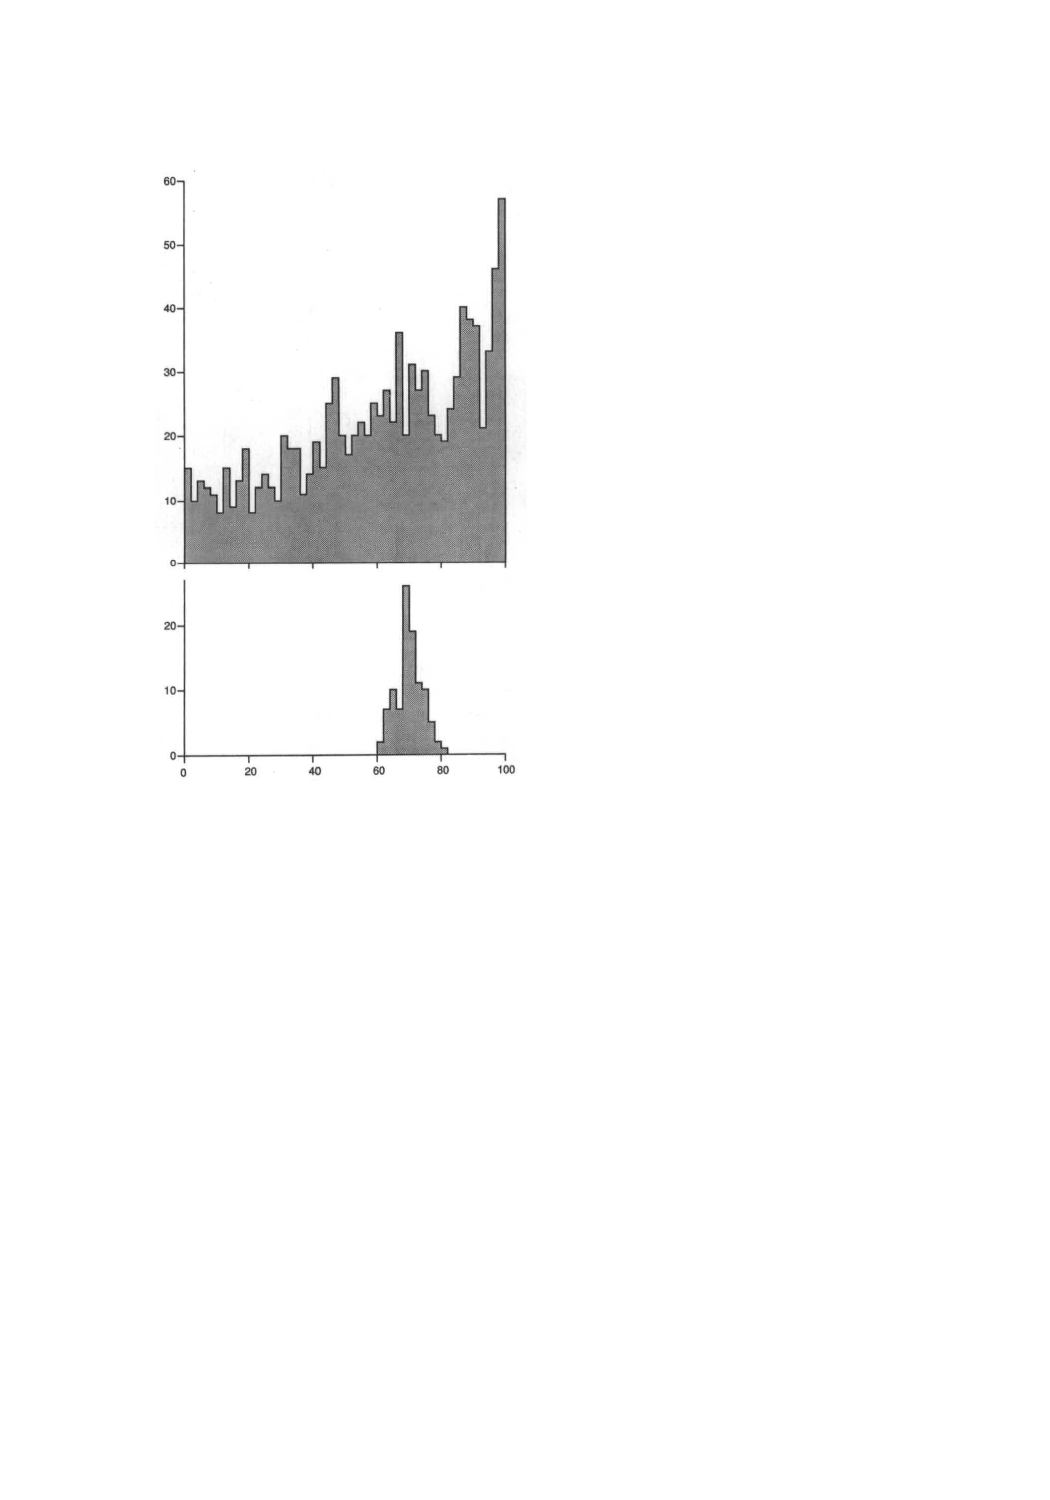
\includegraphics[scale=1.2]{../newimages/HillisB1993Fig3.pdf}}}
      \put(150,-330){\small \% recovering tree}
      \put(0,-20){\small bootstrap}
      \put(0,-50){\small values from}
      \put(0,-80){\small many simulations}
      \put(0,-220){\small repeated}
      \put(0,-250){\small simulation}
      \put(390,-170){Simulation study of }
      \put(390,-200){\citet{HillisB1993} }
\end{picture}


\myNewSlide
\section*{Bootstrap Proportion $\neq$ Posterior Probability}
Several studies have compared the non-parametric bootstrap proportion of clade from an ML analysis of a data set to the posterior probabilities when the same data is analyzed under the same model \citep{SuzukiGN2002,WilcoxZHH2002,AlfaroZL2003,CummingsHMRRW2003,DouadyDBDD2003}.\par

Note: {\em \bf Not} all of these have implied that the measures {\em\bf should} be the same, but some authors have \citep[usually citing][]{EfronHH1996}.

\myNewSlide
\section*{Bootstrap Proportion $\neq$ Posterior Probability in general}
\begin{picture}(-0,0)(-0,0)
    \put(40,-50){\makebox(30,-150)[l]{\includegraphics[scale=2]{/home/mtholder/Documents/ku_teaching/BIOL-848-2013/images/WilcoxZHH-figure.pdf}}}
    \put(40,-330){from \citet{WilcoxZHH2002}}
    \put(40,-380){\normalsize Note: \citet{HuelsenbeckR2004} showed that the Bayesian posterior probabilities}
    \put(40,-400){\normalsize are right on the equality line, if you  simulate from the prior.}
\end{picture}


\myNewSlide
\section*{\citet{Newton1996} showed that, when you look at the median, the BP may not be biased downward}
\begin{picture}(-0,0)(-0,0)
    \put(40,-50){\makebox(30,-150)[l]{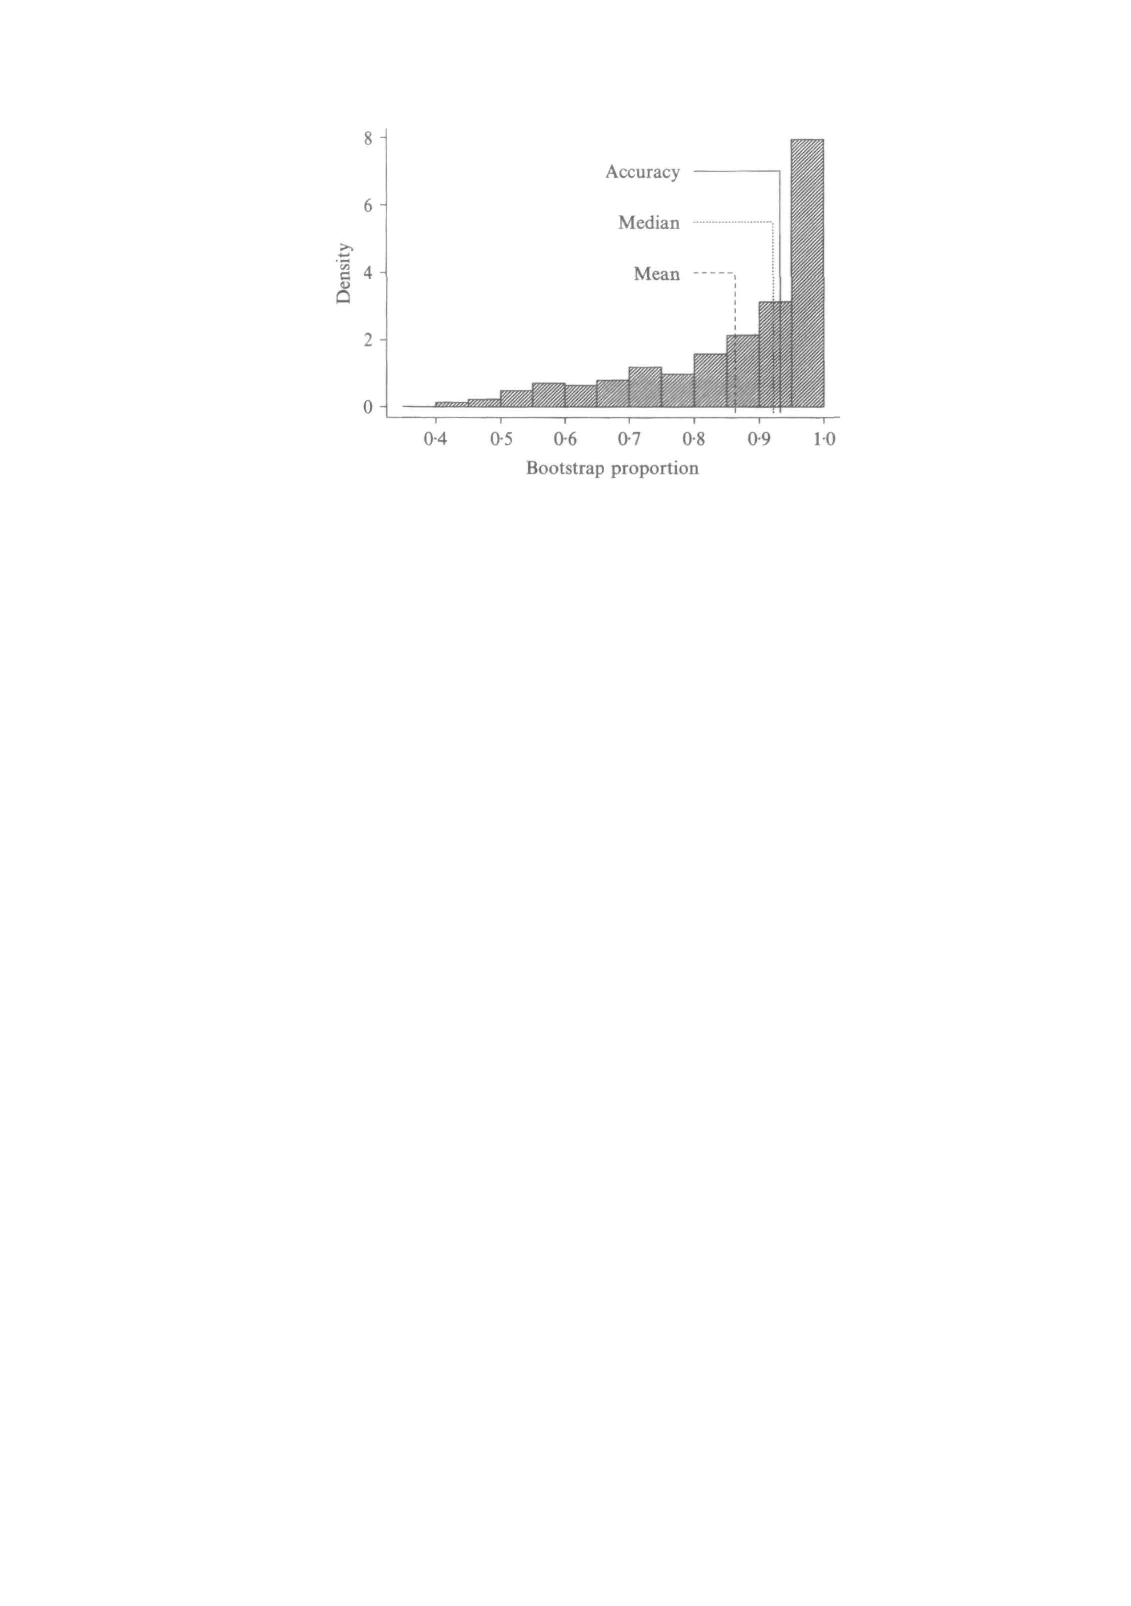
\includegraphics[scale=2]{../newimages/Newton1996Fig4.pdf}}}
    \put(40,-330){Figure 4 from \citet{Newton1996}}
\end{picture}

\myNewSlide
\section*{What did \citet{EfronHH1996} say?}
\normalsize
We can use a Bayesian model to show that $\tilde{\alpha}$ is a reasonable 
assessment of the probability that $\mathscr{R}_1$ contains $ \mu$.
Suppose we believe \textit{a priori} that $\mu$ could lie anywhere in the plane with 
equal probability. 
Then having observed $\hat{\mu}$, the \textit{a posteriori} 
distribution of  $\mu$ given  $\hat{\mu}$ is $N_2( \hat{\mu},I)$ exactly the same as the 
bootstrap distribution of $\hat{\mu}^{\ast}$. 
In other words, $\tilde{\alpha}$ is the  \textit{a posteriori}
probability of the event $\mu \in \mathscr{R}_1$, if we begin with an ``uninformative'' prior density for $\mu$.
\begin{picture}(-0,0)(-0,0)
    \put(0,-120){\makebox(30,-150)[l]{\includegraphics[scale=4]{/home/mtholder/Documents/ku_teaching/BIOL-848-2013/images/EfronHH-straight-fig.pdf}}}
\end{picture}

\myNewSlide
\section*{\citet{EfronHH1996} view of tree space}
\begin{picture}(-0,0)(-0,0)
    \put(-10,-90){\makebox(30,-150)[l]{\includegraphics[scale=3]{/home/mtholder/Documents/ku_teaching/BIOL-848-2013/images/EfronHH-treespace-fig.pdf}}}
\end{picture}



\myNewSlide
\section*{What did \citet{EfronHH1996} say (and mean)?}
\begin{itemize}
    \item the ``uninformative'' prior density is a uniform prior over all of pattern frequency space
    \item this is {\em not} equivalent to a prior that would be expected to yield a phylogeny (it is actually identical to the prior you would get if you assumed that all pairwise distances between taxa were $\infty$),
    \item  \citet{EfronHH1996}  were {\em not} predicting that the bootstrap proportions should be identical to those from a Bayesian phylogenetic analysis with real phylogenetic priors.
    \item  \cite{SvennbladEOB2006} have a nice paper on this subject.
\end{itemize}


\myNewSlide
\section*{\citet{Newton1996} provides an intuition for why the mean BP may be lower than repeatability}
\begin{picture}(-0,0)(-0,0)
    \put(40,-50){\makebox(30,-150)[l]{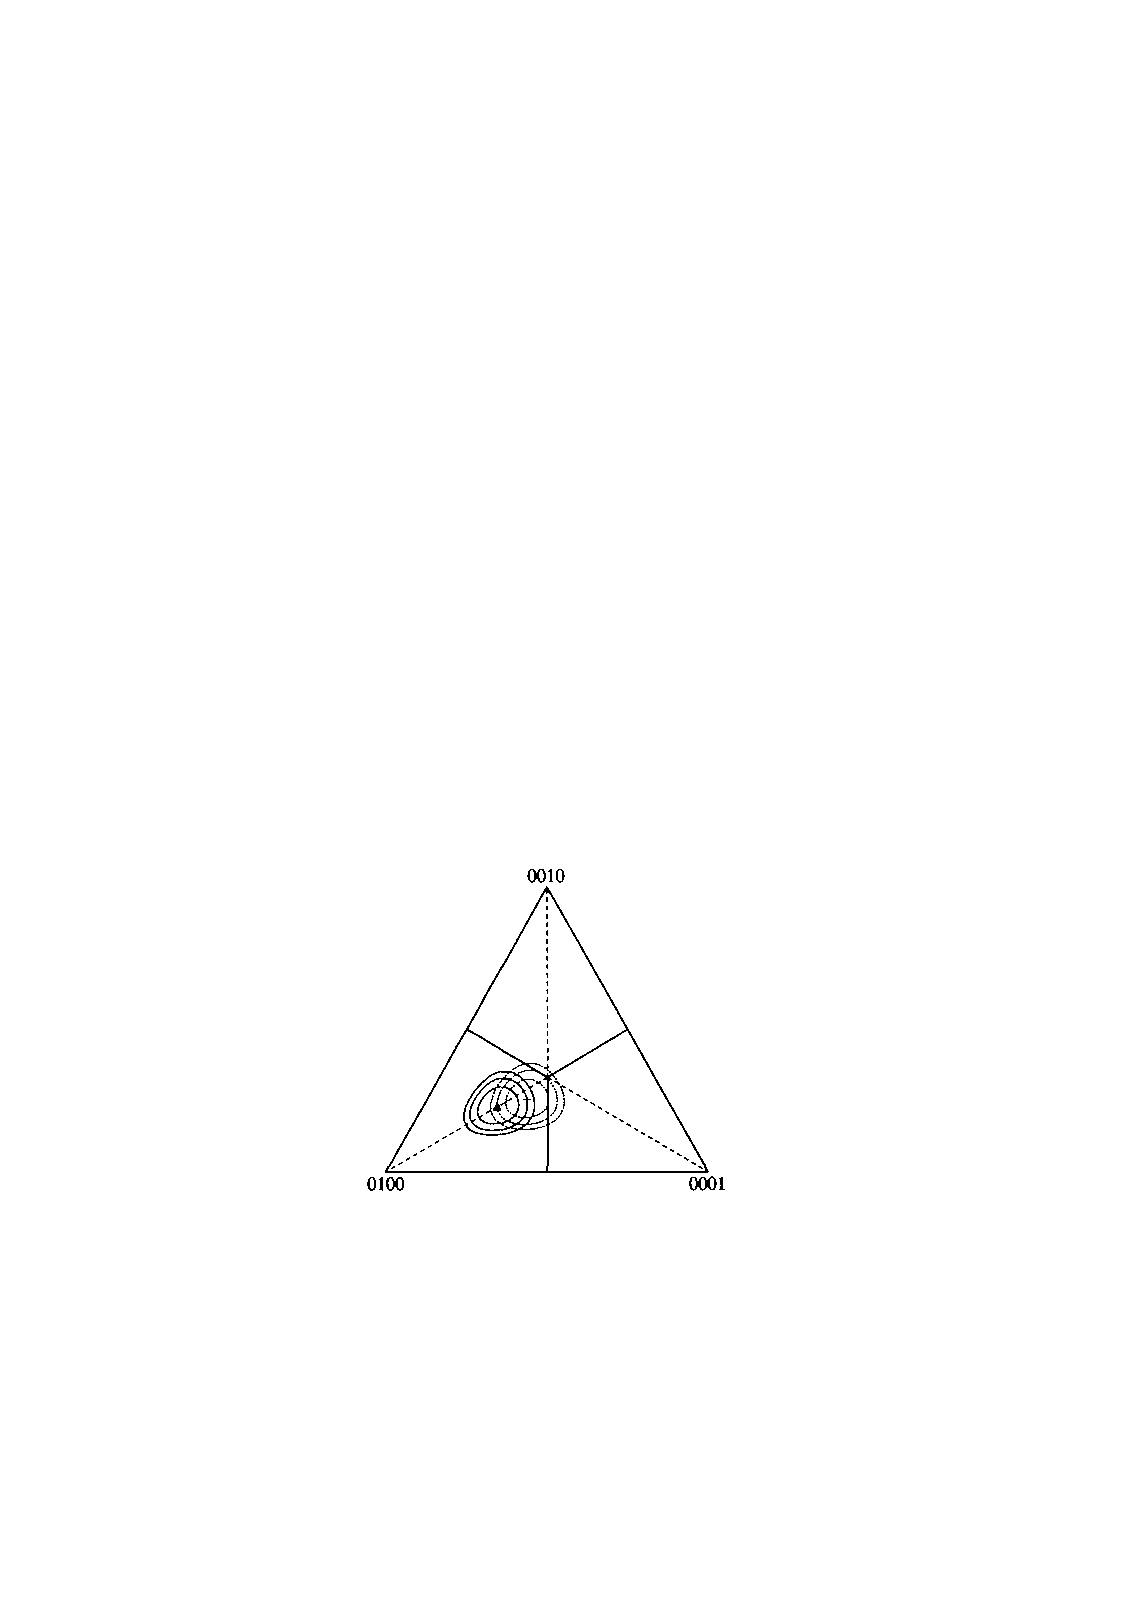
\includegraphics[scale=2]{../newimages/Newton1996Fig3.pdf}}}
    \put(40,-320){Darker ovals indicate probability contours for datasets given the truth}
    \put(60,-350){(note that repeatability $\approx$ 100\%)}
    \put(40,-380){Lighter ovals show probability contours for bootstrapping for one dataset.}
    \put(60,-410){Many real datasets will have BP much $<$ 100\%}
    \put(-40,-50){Figure 3 from \citet{Newton1996}}
\end{picture}



\includepdf[pages={28-45}]{/home/mtholder/Documents/ku_teaching/BIOL-848-2013/lec16-Bootstrapping/lec16Bootstrapping.pdf} 


\myNewSlide
\section*{RELL bootstrap}
\large
Often, the MLE of numerical parameters (including branch lengths) do not change much when we bootstrap.

So, we can simply resample the site $\ln L$ values and sum them (rather than reoptimizing parameters).

This is called the RELL bootstrap \citep[][and Felsenstein]{KishinoMH1990}. It is not a ``safe'' replacement for normal bootstrapping \citep[especially on large trees;][]{StamatakisHR2008} when you want to estimate clade support.

But it should be good enough for helping us learn about the standard error of the $\ln L$.

And it is really fast.




\myNewSlide
\section*{SH test candidate set selection}
\large
\begin{itemize}
    \item Should be all trees that you would have seriously entertained before seeing the data (considering a subset of trees for computational convenience can invalidate the test).
    \item Using all trees is safe.
    \item If a tree has low $\ln L$ and low variance of site-log-likelihoods then it can probably be safely removed without affecting the $P$-values of other trees\footnote{Because such a tree would be unlikely to ever be the tree that is the determines the maximum diplacement from the centered value, $m^{(j)}$.}
\end{itemize}

\myNewSlide
{\bf SH Test details}
\normalsize
\begin{compactitem}
    \item For each tree $T_i$ in the candidate set calculate $\delta(\hat{T}, T_i \mid X)$
    \item Bootstrap to generate ${\ln L}(T_i \mid X^{(j)})$ for each bootstrap replicate $j$.
    \item For each tree $T_i$, use the mean, $\bar{\ln L}(T_i \mid X^{\ast})$, over all bootstrap replicates to center the bootstrapped collection of log-likelihoods:
        $$c_i^{(j)} = {\ln L}(T_i \mid X^{(j)})-\bar{\ln L}(T_i \mid X^{\ast})$$
    \item For each bootstrap replicate, $j$, pick the highest value from the centered distributions (this mimics the selection bias): $$m^{(j)} = \max\left[c_i^{(j)}\right] \mbox{ over all } i$$
    \item Then for each tree and replicate, you get a sample from the null $\delta_i^{(j)} = m^{(j)} - c_i^{(j)}$
    \item $P$-value for tree $T_i$ is approximated by the proportions of bootstrap reps for which: $$\delta_i^{(j)} \geq \delta(\hat{T}, T_i \mid X)$$
\end{compactitem}



\begin{itemize}
    \item $\delta(T_1,T_2 \mid X) = 2\left[\ln L(T_1 \mid X) - \ln L(T_2 \mid X)\right]$ is a powerful statistic for discrimination between trees.
    \item We can assess confidence by considering the variance in signal between different characters.
    \item Bootstrapping helps us assess the variance in $\ln L$ that we would expect to result from sampling error.
\end{itemize}

\myNewSlide
\section*{Summary - Part 2}
\normalsize
A (very) wide variety of tests differ by:
\begin{itemize}
    \item Null hypotheses:
    \begin{compactitem}
        \item Expected scores are the same $\rightarrow$ boundary tests. {\bf Non-parametric tests}
        \item A tree consistent with the null is correct $\rightarrow$ tests that use the full info of the model. {\bf Parametric tests}
    \end{compactitem}
    \item How to use variance information:
    \begin{compactitem}
        \item Rely on ``raw'' bootstrap variability,
        \item Invoke assumptions of normality of scores,
        \item Use $\chi^2$ variants.
    \end{compactitem}
    \item Whether or not the trees must be specified {\em a priori} -- KH Test requires the trees to be specified {\em a priori}.
\end{itemize}

\myNewSlide
\section*{Summary - Part 3}
\large
\begin{table}[htdp]
\begin{center}
\begin{tabular}{|c|p{7cm}|p{6cm}|}
\hline
& Parametric & Nonparametric \\
\hline
$P$-value from $\delta$  & aLRT, aBayes, parametric bootstrapping & KH, SH \\
\hline
$P$-value from BP  &aBP(semi)  & BP, aBP(semi), AU, EHH\\
\hline
\end{tabular}
\end{center}
\label{default}
\end{table}%

When you use a parametric test, you will usually gain power. But non-parametric tests are more robust to model violation.


